\documentclass{article}

\usepackage{icml2026}
\usepackage{amsmath}
\usepackage{amssymb}
\usepackage{booktabs}
\usepackage{graphicx}
\usepackage{multirow}
\usepackage{adjustbox}
\usepackage{hyperref}
\usepackage{url}
\usepackage{enumitem}
\setlist[itemize]{topsep=2pt,itemsep=2pt,parsep=0pt,partopsep=0pt,leftmargin=*}
\setlist[enumerate]{topsep=2pt,itemsep=2pt,parsep=0pt,partopsep=0pt,leftmargin=*}
\graphicspath{{assets/plots/}{assets/media/}}

\icmltitlerunning{SAGE-Mem: Write-Time Governance for Multimodal Agent Memory in Noisy, Low-Trust Environments}

\begin{document}

\twocolumn[
\icmltitle{SAGE-Mem: Write-Time Governance for Multimodal Agent Memory in Noisy and Low-Trust Environments}

\begin{icmlauthorlist}
\icmlauthor{Anonymous Author}{}
\end{icmlauthorlist}

\icmlaffiliation{}{Anonymous Institution}

\icmlkeywords{multimodal agents, low-resource ML, Global South, memory safety, adversarial robustness}

\vskip 0.3in
]

\printAffiliationsAndNotice{}



\begin{abstract}
ML systems deployed in low-resource and low-trust environments must process noisy OCR, low-quality images, multilingual text, and unverified web outputs under limited human oversight. In such settings, memory corruption is consequential: once unsupported content enters persistent memory, it can distort decisions long after the original input has disappeared. We study \textbf{write-time governed multimodal memory} as a robustness mechanism for these environments. We present \textbf{SAGE-Mem}, a memory layer that combines typed memory stores for \emph{evidence}, \emph{belief}, and \emph{control}, guard-based admission, Bayesian source trust, anomaly-aware write filtering, dependence-aware belief promotion, provenance-aware retrieval, and an optional LLM-based fallback guard for borderline write decisions. To evaluate this setting, we construct an adversarial-and-noisy multimodal extension of LoCoMo-10 with poisoning, Visual Prompt Injection (VPI), and missing-modality stress, and pair it with an adversarial MM-BrowseComp benchmark used as a proxy for low-trust web and document ecosystems. On the LoCoMo extension, SAGE-Mem reduces write admission and retrieval contamination to near-zero, but yields lower benign utility than a retrieval-time baseline, exposing a clear integrity--utility tradeoff. On MM-BrowseComp, a provenance prior alone is insufficient for browser-sourced overwrite attacks, motivating \textbf{SAGE-Mem-BrowseGuard}, a browser-specific write-time gate that combines typed claim control with composite semantic suspicion scoring over page-local and memory-context signals. On a 194-case adversarial benchmark with 388 overwrite attempts, SAGE-Mem-BrowseGuard achieves zero write admission and zero retrieval contamination while preserving near-clean utility. These results show that \textbf{write-time governance is a practical complement to retrieval-time filtering for multimodal memory in noisy, low-trust deployments}, especially when apparently corroborating multimodal signals are actually dependent views of the same corrupted source.
\end{abstract}

\section{Introduction}

Across many real-world deployments, especially in low-resource settings, ML systems do not operate on clean, trusted, or fully curated streams of information. They ingest scanned forms with OCR noise, low-quality phone images, multilingual and code-switched text, scraped web evidence, and tool outputs of varying reliability. In public-sector, healthcare, logistics, education, and digital public infrastructure applications, such systems increasingly rely on persistent memory to maintain context over long horizons. That same persistence turns unreliable observations into durable risk: once unsupported content is stored, it can be resurfaced, summarized, and reused long after the original input has disappeared.

Memory poisoning is therefore especially consequential in low-trust information ecosystems. A stateless model can be manipulated only within the current context window; a stateful system can be manipulated by altering the persistent memory that future reasoning depends on. In environments where verification is expensive, bandwidth is limited, and trusted human review is intermittent, misinformation that becomes persistent state may be much harder to detect and correct.

This matters even more for multimodal systems. OCR text, vision captions, browser outputs, and user or tool messages are not interchangeable evidence channels. A single adversarial image can generate both OCR text and a caption-like description, creating the appearance of corroboration even though both observations derive from the same corrupted source. For persistent memory, this kind of \textbf{dependent corruption} matters as much as direct prompt injection.

Our claim is deliberately narrow. We do not attempt full multimodal truth inference. Instead, we ask a systems question that matters immediately for deployed agents: \emph{when should heterogeneous multimodal observations be allowed to become persistent state, when should they remain weak evidence, and when should apparent cross-modal agreement be discounted because it comes from the same source object?}

Most existing defenses address this question too late. Retrieval-time reliability scoring can reduce the chance that a poisoned item is surfaced, but it does not restore the memory state once unsupported content has been admitted. In resource-constrained deployments, a permissive memory store creates three downstream costs:

\begin{enumerate}
\item \textbf{State corruption:} the store contains observations that should never have been admitted.
\item \textbf{Retrieval burden:} reranking and filtering must repeatedly separate signal from contamination.
\item \textbf{Compounding distortion:} later summaries and derived beliefs may inherit unsupported content.
\end{enumerate}

We therefore study \textbf{write-time governance} as the primary intervention point and evaluate it with \textbf{lifecycle metrics}, not only final QA accuracy. The relevant questions are whether an attack is admitted, whether it hardens into belief, whether it resurfaces at retrieval, and what benign utility is preserved under that policy. Our system, \textbf{SAGE-Mem}, implements this view through guard-based admission, Bayesian source trust, anomaly-aware write filtering, typed memory stores, dependence-aware belief promotion, and provenance-aware retrieval. We evaluate SAGE-Mem on a controlled adversarial-and-noisy multimodal extension of LoCoMo-10 that we construct for this paper, and on an adversarial browsing benchmark derived from MM-BrowseComp. This framing is particularly relevant in deployments where memory integrity matters more than maximizing short-term answer rate.

\subsection{Why Write-Time Defense Is Distinct}

Retrieval-time filtering and write-time governance solve different problems. Retrieval-time defense asks which items should be surfaced from a possibly contaminated store. Write-time defense asks which observations should be allowed to become persistent state in the first place.

The second question is harder for three reasons:

\begin{enumerate}
\item \textbf{Partial observability at ingestion time.} The system must decide before it has future context.
\item \textbf{Memory-state externalities.} A write-time mistake changes later retrieval, summarization, and consolidation.
\item \textbf{Multimodal dependence.} Apparent agreement between channels may be duplicated evidence from one source rather than independent support.
\end{enumerate}

These differences motivate our evaluation protocol. A write-time defense should not be judged only by final-answer accuracy, because write admission, belief formation, and retrieval contamination expose distinct failure modes. They also motivate how we compare against retrieval-time baselines such as MMA: the goal is not a single leaderboard ranking, but an \textbf{integrity--utility frontier}. Retrieval-time methods favor short-term answer utility from a broad memory store; write-time governance favors memory-state integrity by rejecting unsupported writes, sometimes at the cost of benign recall. That tradeoff is especially relevant in noisy, low-trust deployments where memory corruption can persist for long periods without human correction.

\subsection{Hypotheses}

We test six concrete hypotheses:

\begin{description}[style=nextline,leftmargin=0pt,labelsep=0.4em,font=\normalfont\bfseries]
\item[H1: Write-time governance hypothesis.] Relative to retrieval-time filtering alone, a governed write boundary should reduce attack write admission and retrieval contamination on long-horizon multimodal memory tasks.
\item[H2: Belief-formation hypothesis.] Typed evidence-to-belief promotion should reduce the rate at which unsupported or adversarial observations harden into durable, answer-bearing memory.
\item[H3: Dependent-evidence hypothesis.] Multimodal attacks such as VPI exploit dependence between OCR and caption outputs from the same image; modeling those channels as dependent should improve robustness relative to consensus-style trust.
\item[H4: Noise-calibration hypothesis.] Under noisy or missing modalities, adaptive trust calibration should reduce over-quarantine relative to simpler write-time baselines while preserving low attack survival.
\item[H5: Browsing-context prior hypothesis.] Browsing-derived external tool text is not equivalent to trusted internal tool output. A provenance-aware browser prior should improve robustness relative to generic tool trust without globally lowering trust in all tool outputs. This extension is instantiated as \textbf{SAGE-Mem-Browse}.
\item[H6: Browsing-guard hypothesis.] A browser-specific write-time layer should maintain robustness against adaptive adversaries that bypass a simple provenance prior. \textbf{SAGE-Mem-BrowseGuard} combines typed claim control for browser-sourced \texttt{qa\_answer} writes with composite semantic suspicion scoring over memory conflict, page-group outlierness, corroboration deficit, and channel history, reducing ASR on browsing overwrite attacks while preserving clean utility.
\end{description}

The experiments support H1, H3, H4, and H6; they provide partial support for H2; and they reject H5. That pattern matters for deployment: a provenance prior alone does not protect browsing-derived memory writes, but a browser-specific write policy does.

\subsection{Contributions}

This paper makes four contributions.

\begin{enumerate}
\item \textbf{Write-time framing for unreliable multimodal environments.} We formulate memory poisoning as a write-boundary and belief-boundary problem and show why lifecycle metrics are needed to evaluate it in noisy, low-trust settings.
\item \textbf{SAGE-Mem.} We introduce a governed memory layer with typed memory stores, guard-based admission, Bayesian source trust, anomaly-aware write filtering, dependence-aware promotion, provenance-aware retrieval, and an optional LLM-based fallback guard for borderline write decisions.
\item \textbf{Lifecycle evaluation across two regimes.} We evaluate on an adversarial-and-noisy multimodal extension of LoCoMo-10 that we construct for this paper, and on a browsing benchmark with browser-derived overwrite attacks, using metrics for write admission, belief formation, retrieval contamination, and downstream utility.
\item \textbf{Empirical findings and browser-specific extension.} We show that write-time governance substantially improves memory-state integrity on LoCoMo-style tasks, that a provenance prior alone is insufficient for browser-derived attacks, and that \textbf{SAGE-Mem-BrowseGuard} achieves zero write admission and zero retrieval contamination on the combined MM-BrowseComp adversarial benchmark while preserving near-clean utility.
\end{enumerate}

The central claim is correspondingly scoped: write-time governance strengthens memory-state integrity beyond retrieval-time filtering alone, especially under multimodal corruption, but it does not dominate retrieval-time methods on benign utility. The comparison is a tradeoff, not a claim of universal superiority.

\subsection{Relation to Prior Work}

This paper sits at the intersection of four lines of work. Prior research on memory poisoning shows that persistent memory is a durable attack surface~\cite{ref1,ref2,ref3}. Retrieval-time robustness work studies corrupted context and prompt injection at inference time~\cite{ref4,ref5,ref6,ref7}. Multimodal security work shows that images can manipulate OCR, captioning, and downstream reasoning~\cite{ref8}. Work on memory-augmented agents and long-horizon QA provides the underlying evaluation setting~\cite{ref9,ref10,ref11}. Our contribution is not to reintroduce these problems individually, but to combine them into a single systems question: how should a multimodal memory layer govern \emph{admission}, \emph{belief formation}, and \emph{retrieval} when apparently corroborating observations may be dependent and adversarial?

The paper's novelty lies in three pieces taken together: write-time governed multimodal memory, dependence-aware treatment of multimodal evidence, and lifecycle evaluation that separates write admission, belief formation, retrieval contamination, and downstream utility. This shifts the unit of analysis from the final answer alone to the integrity of the latent memory state that future answers depend on.



\section{Problem Setting}

\subsection{Agentic Memory Pipeline}

We model an agent with persistent memory as a four-stage pipeline:

\begin{enumerate}
\item \textbf{Observation ingestion:} raw observations arrive from channels such as \texttt{tool\_output\_text}, \texttt{ocr\_text}, \texttt{vision\_caption}, or \texttt{user}.
\item \textbf{Memory admission:} the system decides whether to write the observation into planning memory, quarantine it, or place it into an audit partition.
\item \textbf{Belief formation:} accepted evidence may later be summarized or promoted into more durable belief-like memory items.
\item \textbf{Retrieval and downstream use:} later questions retrieve memory items that influence planning or answer generation.
\end{enumerate}

Let \(x_t\) denote the \(t\)-th incoming observation, let \(M_t\) denote the current memory state, and let \(R(q, M_t)\) denote the retrieval set for query \(q\). A write-time defense changes the transition

\[
M_{t+1} = \mathcal{U}(M_t, x_t)
\]

itself, not only the retrieval function \(R\).

\subsection{Threat Model}

The adversary can inject malicious content into external observations that the agent ingests from untrusted channels. In our main threat model, the adversary controls the \textbf{content} of an observation but not the trusted orchestration layer that assigns \texttt{source\_type} and \texttt{channel\_id}.

The attacker may:
\begin{itemize}
\item inject malicious tool outputs or web observations,
\item embed malicious directives in OCR-visible or caption-visible image content,
\item use natural-language corrections that mimic benign content,
\item exploit summarization or consolidation to spread attack lineage.
\end{itemize}

The attacker may \textbf{not}:
\begin{itemize}
\item relabel an arbitrary observation as a higher-trust channel,
\item directly edit the memory store,
\item compromise the orchestrator itself.
\end{itemize}

Trusted-user attacks are treated separately as stress tests, not as part of the main benchmark claim, because authenticated user content is intentionally treated as a trust anchor in the system design.

\subsection{Multimodal Noise and Dependence}

A multimodal memory system is not only vulnerable to adversarial corruption; it is also vulnerable to \textbf{dependence mis-modeling}. Suppose a single image produces two observations:
\begin{itemize}
\item an OCR transcription, and
\item a VLM-generated caption.
\end{itemize}

If both contain the same malicious payload, a naive system may treat them as corroborating evidence. But conditional independence does not hold: both observations are functions of the same adversarial source. This motivates our VPI threat model and the corresponding design principle that \textbf{agreement across dependent channels should not be rewarded as independent support}.



\section{SAGE-Mem}

SAGE-Mem is a governed memory layer between heterogeneous observation sources and a downstream planner. It combines guard-based admission, Bayesian source trust, anomaly-aware write filtering, typed memory stores, and dependence-aware belief promotion. It is not a full agent architecture; its role is to preserve memory-state integrity before later planning and answer generation. Figure~\ref{fig:sagemem-architecture} summarizes the overall write-time pipeline.

\subsection{Typed Memory}

SAGE-Mem separates memory into three partitions:
\begin{itemize}
\item \emph{evidence}: raw or grounded observations,
\item \emph{belief}: more durable, answer-supporting state,
\item \emph{control}: content that could steer policy or action.
\end{itemize}

This separation prevents the system from treating every accepted observation as an equally trustworthy fact. In particular, multimodal observations often begin as weak evidence and should only become durable belief after additional support.

\subsection{Write-Time Admission}

For an observation \(o\) from channel \(c\) and source \(s\), admission is controlled by a conjunction of guard checks:

\begin{equation}
\begin{aligned}
\mathrm{accept}(o)=1 \iff {} & g(o)=\mathrm{DATA} \\
& \wedge\ \theta(c,s)\ge \tau_t \\
& \wedge\ d_M(o)\le \xi_t \\
& \wedge\ \theta_{\mathrm{browser}}(o)\ge \tau_t \\
& \wedge\ \neg \psi_{\mathrm{VPI}}(o) \\
& \wedge\ \neg \mathrm{unsafe\_conflict}(o)
\end{aligned}
\end{equation}

where
\begin{itemize}
\item \(g(o)\) is the write-time semantic guard classification that decides whether a write should be treated as evidence, instruction, or non-evidential page scaffolding,
\item \(\theta(c,s)\) is the Bayesian trust posterior for channel \(c\) and source \(s\),
\item \(d_M(o)\) is the session-relative anomaly score,
\item \(\theta_{\mathrm{browser}}(o)\) is an optional source-context prior for browser-derived external text,
\item \(\psi_{\mathrm{VPI}}(o)\) detects suspicious cross-modal corroboration.
\end{itemize}

In the implementation, this write boundary also supports an optional LLM-based semantic guard fallback. When enabled, a stateless write-time guard or skeptic--advocate ensemble classifies incoming text as \texttt{DATA}, \texttt{DIRECTIVE}, or \texttt{METADATA}; high-risk directive-like content is quarantined before it can enter durable state, while benign \texttt{DATA} can pass downstream with extracted atomic facts. We treat this as a fallback or escalation layer rather than as the core claim of SAGE-Mem, which is the governed write-time architecture itself.

For the reported paper runs, these provenance priors are fixed from the threat model rather than learned from benchmark outcomes. The released configuration assigns higher prior trust to authenticated users and orchestrator-controlled tool output than to browser-derived text, OCR, captions, self-summaries, or echoed content; the exact default values used in the runs are \texttt{user}=1.00, \texttt{tool\_output\_text}=0.70, \texttt{ocr\_text}=0.60, \texttt{vision\_caption}=0.58, \texttt{self\_summary}=0.45, \texttt{browser\_tool\_output\_text}=0.35, and \texttt{tool\_echo}=0.20. The configuration also contains a low-trust \texttt{attacker}=0.10 entry used only for benchmark attack insertions with explicit attacker labels. The codebase supports offline recalibration of these priors on held-out clean data, but all final paper artifacts use the fixed default prior table.

The key architectural choice is the location of this decision. SAGE-Mem attempts to stop unsupported observations \textbf{before} they become persistent state. The browser prior is defined at the provenance level rather than at the benchmark level: generic \texttt{tool\_output\_text} may correspond to trusted internal APIs, while \texttt{browser\_tool\_output\_text} denotes externally controlled page content. This distinction lets us test whether browser failures arise from missing source-context calibration rather than from a generic failure of write-time governance.

\subsection{Belief Promotion}

Admitted evidence is not automatically promoted into belief memory. Promotion is gated by support sufficiency:

\[
\mathrm{promote}(q)=1
\iff
\left|P_{\ge \tau_p}(q)\right| \ge k_s
\wedge
\left|\mathrm{independent}(P_{\ge \tau_p}(q))\right| \ge k_i
\wedge
\neg \mathrm{conflict}(P(q)).
\]

This rule matters because multimodal support can be plentiful without being independent. OCR text and a vision caption from the same image should not count as two independent votes for the same claim. In SAGE-Mem, the promotion boundary is therefore as important as the write boundary.

\subsection{Provenance and Retrieval}

At retrieval time, SAGE-Mem returns answer-supporting memory together with its evidence lineage. We evaluate this with belief traceability and false-belief retrieval. The goal is not only relevance, but also inspectable support for the retrieved belief.

\subsection{System Intent}

The systems motivation is straightforward:
\begin{itemize}
\item less persistent noise in the store,
\item fewer malicious or low-value items consuming token budget,
\item less summary distortion over time,
\item lower burden on retrieval-time reranking.
\end{itemize}

Retrieval-time filtering remains useful, but it acts on an already-evolved memory state. SAGE-Mem is designed to keep that state cleaner to begin with.

\begin{figure*}[t]
\centering
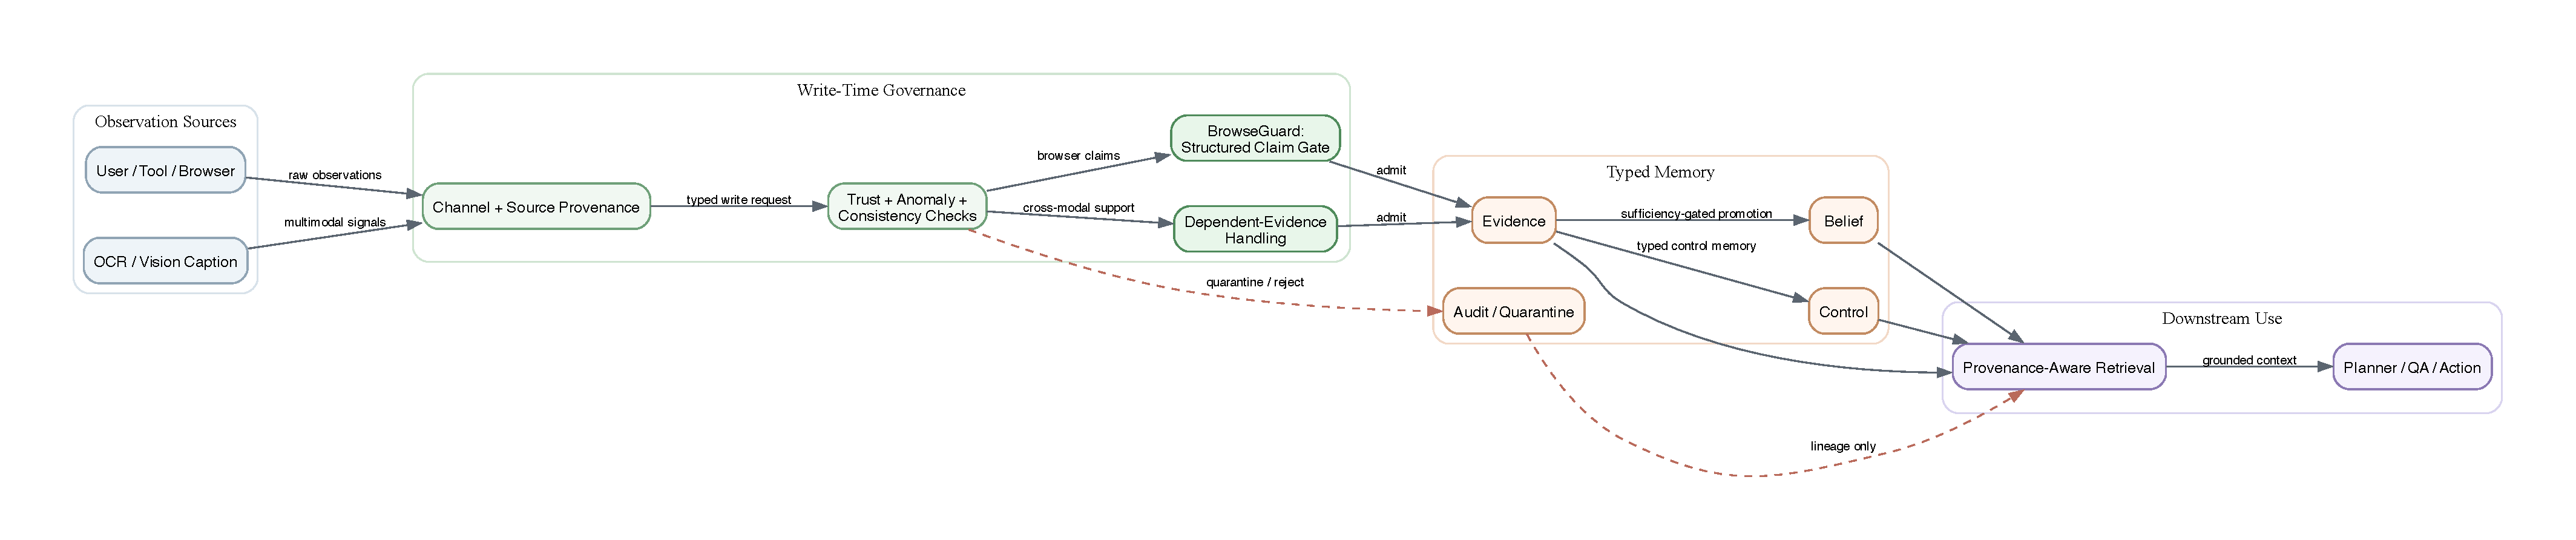
\includegraphics[width=0.92\textwidth]{sagemem_architecture.pdf}
\caption{SAGE-Mem architecture for write-time governed multimodal memory. Heterogeneous observations pass through guard-based admission, Bayesian trust scoring, anomaly-aware filtering, and typed memory stores before retrieval. BrowseGuard extends the write boundary with browser-specific typed claim control and composite semantic suspicion scoring for overwrite attempts, while dependent-evidence handling prevents duplicated multimodal signals from being counted as independent support.}
\label{fig:sagemem-architecture}
\end{figure*}



\section{Evaluation Design}

\subsection{Benchmarks}

We evaluate in two complementary regimes: a controlled long-horizon setting where lifecycle effects can be measured cleanly, and a harder browsing setting that stresses source-context calibration.

\subsubsection{LoCoMo-10 with multimodal adversarial extension}

LoCoMo provides a controlled long-horizon QA benchmark over multi-session conversations. We augment it with multimodal observation writes and adversarial injections. The resulting benchmark is controlled rather than fully naturalistic, but it is well suited for causal analysis of poisoning over long memory lifecycles.

We use three LoCoMo-based settings:
\begin{itemize}
\item \textbf{Main suite:} untrusted-channel memory-poisoning attacks,
\item \textbf{VPI-only suite:} Visual Prompt Injection in isolation,
\item \textbf{multimodal robustness suite:} missing/noisy modality stress.
\end{itemize}

\subsubsection{Adversarially augmented MM-BrowseComp}

We build a browsing-style multimodal memory benchmark from MM-BrowseComp observation traces, augmented with VLM-backed image observations and separate clean and adversarial tracks. This setting is more realistic than the LoCoMo extension as a browsing-memory stress test and is best interpreted as an external evaluation of source-context calibration rather than a standard QA benchmark.

\subsection{Attack Families}

The main LoCoMo suite includes:
\begin{itemize}
\item \texttt{constructor\_launder}
\item \texttt{label\_gaming}
\item \texttt{ocr\_injection}
\item \texttt{vision\_caption\_injection}
\item \texttt{visual\_prompt\_injection}
\item \texttt{fact\_overwrite\_injection}
\item \texttt{adaptive\_nl\_evasion}
\item \texttt{buried\_payload}
\end{itemize}

The MM-BrowseComp adversarial track uses two attack variants:

\begin{itemize}
\item \texttt{fact\_overwrite\_injection}: a direct overwrite attempt that asserts a replacement fact within browser-derived content.
\item \texttt{fact\_overwrite\_adaptive}: a semantically equivalent overwrite attempt expressed differently.
\end{itemize}

Evaluating both variants matters because success on only one wording would indicate brittle overwrite resistance rather than robust defense.

\subsection{Metrics}

We evaluate the memory lifecycle directly. This metric choice is central to the paper: retrieval-time and final-answer metrics alone are insufficient for a system whose main purpose is to keep unsupported observations out of durable state. We therefore measure admission, belief formation, and retrieval contamination before turning to downstream utility.

\subsubsection{Primary mechanism metrics}

\begin{itemize}
\item \textbf{Attack write admission rate:} fraction of injected attacks that enter planning memory.
\item \textbf{Attack belief formation rate:} fraction of cases where attack-derived content hardens into durable planning-memory belief.
\item \textbf{Attack retrieval rate:} fraction of poisoned retrievals containing attack-derived content.
\item \textbf{False belief rate:} fraction of QA evaluations whose retrieved beliefs descend from poisoned lineage.
\end{itemize}

\subsubsection{Primary downstream utility metric}

\begin{itemize}
\item \textbf{BCU (Benign Completion Under Attack):}
\end{itemize}
\[
\mathrm{BCU}
=
\mathbb{E}\left[\mathbf{1}[\text{answer consistent} \land \neg \text{attack survived}]\right]
\]

This is a per-QA joint metric. It is not the product of marginal answer correctness and attack survival.

\subsubsection{Secondary metrics}

\begin{itemize}
\item \textbf{ASR:} retrieval-time attack survival.
\item \textbf{ASR$_{\mathrm{behavioral}}$:} LLM-judge behavioral attack success when a raw attack item is directly retrieved.
\item \textbf{Belief traceability:} mean fraction of retrieved belief items with usable support lineage; reported as N/A when no belief items are retrieved.
\end{itemize}

For the frozen LoCoMo main and VPI runs, we additionally use an external LLM judge for behavioral attack survival and answer entailment. The judge sees only the retrieved memory context, question, and gold answer; it does not receive attack metadata, channel labels, or benchmark-specific triggers. This complements exact-match-style metrics with a stronger semantic check of attack survival and answer entailment. The canonical MM-BrowseComp tables use lifecycle metrics without LLM-judge evaluation.

\subsection{Compared Conditions}

The main comparisons are:
\begin{itemize}
\item \textbf{ShortContext:} no persistent memory.
\item \textbf{MMA:} retrieval-time reliability scoring baseline.
\item \textbf{RSum:} consolidation baseline without guard.
\item \textbf{H1 / H2 / H3:} mechanism-level internal baselines.
\item \textbf{SAGE-Mem:} final combined governed-memory method.
\end{itemize}

The key comparison is therefore \textbf{retrieval-time filtering versus write-time governed memory}, with ablations that isolate which components matter in each regime.

\subsection{Implementation Notes}

All reported paper results use one fixed SAGE-Mem configuration across benchmarks, including the same provenance-prior table described in Section~3.2; we do not retune those priors separately for LoCoMo, VPI, noisy-modality stress, or MM-BrowseComp. The Pareto plots in Figures~\ref{fig:pareto-locomo} and~\ref{fig:pareto-browsing} are generated directly from the same frozen benchmark summaries that underlie the main LoCoMo and MM-BrowseComp tables, rather than from a separate tuning sweep.



\section{Results}

\subsection{Main LoCoMo Result}

\begin{table}[t]
\centering
\small
\setlength{\tabcolsep}{3.5pt}
\renewcommand{\arraystretch}{0.96}
\begin{adjustbox}{max width=\columnwidth}
\begin{tabular}{lrrrrrr}
\toprule
Method & BCU clean & BCU poison & Write ASR & Belief ASR & Retrieval ASR & False belief \\
\midrule
MMA & 0.7500 & 0.6417 & 1.0000 & 0.0000 & 0.1333 & 0.0000 \\
RSum & 0.4050 & 0.4533 & 0.0000 & 0.0000 & 0.0067 & 0.0000 \\
H1 & 0.3950 & 0.4517 & 0.0000 & 0.0000 & 0.0033 & 0.0000 \\
H2 & 0.3850 & 0.4533 & 0.0000 & 0.0000 & 0.0017 & 0.0000 \\
H3 & 0.2400 & 0.2133 & 0.0000 & 0.0000 & 0.0667 & 0.0000 \\
\textbf{SAGE-Mem} & \textbf{0.3950} & \textbf{0.4600} & \textbf{0.0000} & \textbf{0.0000} & \textbf{0.0000} & \textbf{0.0000} \\
\bottomrule
\end{tabular}
\end{adjustbox}
\caption{Main LoCoMo result. SAGE-Mem eliminates write admission and retrieval contamination on the primary long-horizon benchmark, while MMA preserves substantially higher benign utility.}
\label{tab:locomo-main}
\end{table}


\paragraph{Interpretation.}
Table~\ref{tab:locomo-main} establishes the central tradeoff in the paper. SAGE-Mem eliminates attack write admission and retrieval contamination on the main LoCoMo suite, while MMA preserves much higher benign utility. The comparison is therefore not ``which method wins overall,'' but which operating point is preferable: a cleaner persistent store with lower attack survival, or a more permissive store with higher short-term utility.

\paragraph{Seed stability.}
Across multiple seeds, MMA achieves BCU$_\text{poison}=0.655 \pm 0.015$ with ASR $= 0.158 \pm 0.018$ and Write ASR $= 1.0$. SAGE-Mem achieves BCU$_\text{poison}=0.418 \pm 0.006$, ASR $= 0.0$, and Write ASR $= 0.004 \pm 0.007$. The zero-ASR result is stable across seeds.

\paragraph{Per-attack behavior.}
SAGE-Mem completely blocks six of the seven logged attack families at write time (\texttt{adaptive\_nl\_evasion}, \texttt{constructor\_launder}, \texttt{fact\_overwrite\_injection}, \texttt{label\_gaming}, \texttt{vision\_caption\_injection}, and \texttt{visual\_prompt\_injection}). The sole residual is \texttt{ocr\_injection} at Write ASR = 0.033, but this attack does not survive to retrieval. MMA admits every attack family with Write ASR = 1.0; retrieval contamination is highest on \texttt{fact\_overwrite\_injection} (0.085), \texttt{adaptive\_nl\_evasion} (0.078), and \texttt{visual\_prompt\_injection} (0.078).

\paragraph{Benign-write retention.}
The utility gap has a clear mechanistic cause. On the poisoned LoCoMo main suite, overall benign write recall is 0.010 for SAGE-Mem versus 1.0 for MMA; answer-supporting benign write recall is 0.007 versus 1.0. The current SAGE-Mem configuration is therefore highly conservative: it blocks attacks effectively, but it also rejects too much benign evidence.

\subsection{Visual Prompt Injection}

The VPI setting isolates the multimodal dependence hypothesis with the clearest signal.

\begin{table}[t]
\centering
\small
\setlength{\tabcolsep}{3.8pt}
\renewcommand{\arraystretch}{0.96}
\begin{adjustbox}{max width=\columnwidth}
\begin{tabular}{lrrrrr}
\toprule
Method & BCU clean & BCU poison & Write ASR & Retrieval ASR & ASR \\
\midrule
MMA & 0.7650 & 0.7117 & 1.0000 & 0.0700 & 0.0700 \\
RSum & 0.3800 & 0.3900 & 0.0000 & 0.0000 & 0.0000 \\
H1 & 0.3700 & 0.3800 & 0.0000 & 0.0000 & 0.0000 \\
H2 & 0.3700 & 0.3700 & 0.0000 & 0.0000 & 0.0000 \\
H3 & 0.2400 & 0.2700 & 0.0000 & 0.0000 & 0.0000 \\
\textbf{SAGE-Mem} & \textbf{0.3800} & \textbf{0.3800} & \textbf{0.0000} & \textbf{0.0000} & \textbf{0.0000} \\
\bottomrule
\end{tabular}
\end{adjustbox}
\caption{Visual Prompt Injection (VPI) results. SAGE-Mem fully suppresses write admission and retrieval contamination in the current VPI regime, supporting the dependent-evidence design.}
\label{tab:locomo-vpi}
\end{table}


\paragraph{Interpretation.}
The VPI experiment isolates the dependence argument cleanly. MMA retains higher utility but admits every attack write, whereas SAGE-Mem suppresses both write admission and retrieval contamination. This supports the specific claim that OCR and caption outputs from the same image should not be treated as independent corroboration.

\subsection{Noisy/Missing-Modality Robustness}

This experiment tests whether the full architecture degrades gracefully under impaired perception.

\begin{table}[t]
\centering
\small
\setlength{\tabcolsep}{3.5pt}
\renewcommand{\arraystretch}{0.96}
\begin{adjustbox}{max width=\columnwidth}
\begin{tabular}{lrrrrrr}
\toprule
Method & BCU clean & BCU poison & Write ASR & Belief ASR & Retrieval ASR & ASR \\
\midrule
MMA & 0.7117 & 0.5483 & 1.0000 & 0.0000 & 0.2600 & 0.2600 \\
H1 & 0.3983 & 0.4500 & 0.0000 & 0.0000 & 0.0000 & 0.0000 \\
H2 & 0.3917 & 0.4450 & 0.0000 & 0.1000 & 0.0000 & 0.0000 \\
H3 & 0.2500 & 0.2300 & 0.0111 & 0.1000 & 0.1000 & 0.1000 \\
NoBayes & 0.3950 & 0.4433 & 0.0000 & 0.0000 & 0.0000 & 0.0000 \\
NoAnom & 0.3950 & 0.4450 & 0.0000 & 0.0000 & 0.0000 & 0.0000 \\
NoCons & 0.3967 & 0.4433 & 0.0000 & 0.0000 & 0.0000 & 0.0000 \\
\textbf{SAGE-Mem} & \textbf{0.3950} & \textbf{0.4367} & \textbf{0.0111} & \textbf{0.0000} & \textbf{0.0050} & \textbf{0.0050} \\
\bottomrule
\end{tabular}
\end{adjustbox}
\caption{Noisy/missing-modality robustness. The full SAGE-Mem stack maintains near-zero contamination under degraded multimodal evidence, with Bayes-style trust calibration improving robustness to over-quarantine.}
\label{tab:locomo-noisy}
\end{table}


\paragraph{Interpretation.}
Under noisy or missing modalities, SAGE-Mem remains near-zero on retrieval contamination while H3 degrades more noticeably. The Bayes component matters primarily through calibration: it does not transform attack survival, but it reduces over-quarantine relative to \texttt{NoBayes}. This is the clearest evidence that the full stack is not merely a static blocker, but a calibration mechanism for uncertain multimodal inputs.

\subsection{Internal Ablations}

On the main suite, the named ablations do not separate strongly. \texttt{NoBayes}, \texttt{NoAnomaly}, \texttt{NoConsistency}, and full SAGE-Mem are nearly identical on both integrity and utility metrics:

\begin{table}[t]
\centering
\small
\setlength{\tabcolsep}{4pt}
\renewcommand{\arraystretch}{0.96}
\begin{adjustbox}{max width=\columnwidth}
\begin{tabular}{lrrrrr}
\toprule
Method & BCU clean & BCU poison & Write ASR & Retrieval ASR & ASR \\
\midrule
NoBayes & 0.3900 & 0.4350 & 0.0000 & 0.0000 & 0.0000 \\
NoAnomaly & 0.3900 & 0.4350 & 0.0000 & 0.0000 & 0.0000 \\
NoConsistency & 0.3900 & 0.4350 & 0.0000 & 0.0000 & 0.0000 \\
\textbf{SAGE-Mem} & \textbf{0.3900} & \textbf{0.4350} & \textbf{0.0000} & \textbf{0.0000} & \textbf{0.0000} \\
\bottomrule
\end{tabular}
\end{adjustbox}
\caption{Internal ablations on the main LoCoMo suite. The full SAGE-Mem stack and the named ablations are nearly indistinguishable on the main benchmark, indicating that submodule separability is benchmark-dependent.}
\label{tab:locomo-ablations}
\end{table}


The appropriate conclusion is narrower: the governed-memory design is supported on the main suite, but submodule separability is benchmark-dependent, and Bayes-style calibration is best justified by the noisy-modality experiment rather than by the main benchmark.

\subsection{MM-BrowseComp: Clean vs Adversarial}

We evaluate on a 194-case leakage-clean MM-BrowseComp pool. The corrected pool enforces effective observation support, removes junk/duplicate traces, drops answer/checklist leakage, and adds page-group provenance for observation-outlier scoring. The adversarial track includes both \texttt{fact\_overwrite\_injection} and \texttt{fact\_overwrite\_adaptive} in each case, providing two overwrite attempts per case.

\subsubsection{Clean MM-BrowseComp (n=194)}

\begin{table}[t]
\centering
\small
\setlength{\tabcolsep}{5pt}
\renewcommand{\arraystretch}{0.96}
\begin{adjustbox}{max width=\columnwidth}
\begin{tabular}{lr}
\toprule
Method & BCU clean \\
\midrule
ShortContext & 0.1907 \\
MMA & 0.1959 \\
RSum & 0.1804 \\
H1 & 0.1598 \\
SAGE-Mem & 0.1649 \\
SAGE-Mem-Browse & 0.1598 \\
\textbf{SAGE-Mem-BrowseGuard} & \textbf{0.1598} \\
\bottomrule
\end{tabular}
\end{adjustbox}
\caption{Clean MM-BrowseComp utility. All attack metrics are zero on the clean split; differences reflect only benign utility on the browsing benchmark.}
\label{tab:mmbrowse-clean}
\end{table}


All methods achieve zero attack metrics on the clean split. MMA leads on BCU\_clean (0.1959), consistent with the LoCoMo pattern, while the browsing-specific variants incur a small clean-utility cost.

\subsubsection{Adversarial MM-BrowseComp — combined attack (n=194, 388 attack write attempts)}

\emph{Each case receives both \texttt{fact\_overwrite\_injection} and \texttt{fact\_overwrite\_adaptive}, providing two semantically similar overwrite attempts.}

\begin{table}[t]
\centering
\small
\setlength{\tabcolsep}{3.8pt}
\renewcommand{\arraystretch}{0.96}
\begin{adjustbox}{max width=\columnwidth}
\begin{tabular}{lrrrrr}
\toprule
Method & BCU poison & Write ASR & Retrieval ASR & ASR & False belief rate \\
\midrule
ShortContext & 0.0430 & 0.6881 & 0.7938 & 0.7938 & 0.0000 \\
MMA & 0.0000 & 1.0000 & 1.0000 & 1.0000 & 0.0000 \\
RSum & 0.1065 & 0.6314 & 0.8247 & 0.8247 & 0.0000 \\
H1 & 0.1031 & 0.4897 & 0.8316 & 0.8316 & 0.0000 \\
SAGE-Mem & 0.2027 & 0.6521 & 0.5653 & 0.5653 & 0.0773 \\
SAGE-Mem-Browse & 0.0189 & 0.6521 & 0.6907 & 0.6907 & 0.0000 \\
\textbf{SAGE-Mem-BrowseGuard} & \textbf{0.1546} & \textbf{0.0000} & \textbf{0.0000} & \textbf{0.0000} & \textbf{0.0000} \\
\bottomrule
\end{tabular}
\end{adjustbox}
\caption{Adversarial MM-BrowseComp results on the combined overwrite track. BrowseGuard achieves zero write admission and zero retrieval contamination while maintaining near-clean utility, whereas a provenance prior alone does not protect the write boundary.}
\label{tab:mmbrowse-adv}
\end{table}


The browsing results in Table~\ref{tab:mmbrowse-adv} differ sharply from LoCoMo. A provenance prior alone does not solve browser-derived overwrite attacks: \textbf{SAGE-Mem-Browse} is nearly identical to generic SAGE-Mem on write admission (Write ASR = 0.6521), showing that browser provenance by itself is too weak. By contrast, \textbf{SAGE-Mem-BrowseGuard} blocks all 388 attack writes and drives both retrieval contamination and ASR to zero. Its utility under attack remains close to clean performance (BCU\_poison = 0.1546 versus BCU\_clean = 0.1598), whereas MMA collapses to BCU\_poison = 0.0000 under full contamination.

Generic SAGE-Mem without the browser-specific gate still reduces ASR relative to MMA (0.5653 versus 1.0000), but it admits most attacks and produces a false-belief rate of 0.0773. This is the strongest evidence in the paper for the belief-promotion story: once overwrite content enters memory, some of it hardens into durable false belief. A secondary rerun with semantic observation-group scoring does not change this conclusion; it increases page-local anomaly activity, but the structured browser claim gate remains the dominant mechanism.

\paragraph{Seed stability.}
Across seeds, SAGE-Mem-BrowseGuard achieves BCU$_\text{poison} = 0.1546 \pm 0.0000$, ASR $= 0.0 \pm 0.0$, and Write ASR $= 0.0 \pm 0.0$. SAGE-Mem-Browse remains weak under both attack variants with BCU$_\text{poison} = 0.0189 \pm 0.0107$, ASR $= 0.6907 \pm 0.0186$, and Write ASR $= 0.6512 \pm 0.0039$. Generic SAGE-Mem without browser-specific claim typing has better utility (BCU$_\text{poison} = 0.2027 \pm 0.0149$) but remains heavily contaminated (ASR $= 0.5653 \pm 0.0166$, Write ASR $= 0.6512 \pm 0.0039$).

\paragraph{Per-attack breakdown.}
The focused rerun shows that SAGE-Mem-Browse admits both overwrite variants at similarly high rates: Write ASR is 0.6426 on \texttt{fact\_overwrite\_injection} and 0.6598 on \texttt{fact\_overwrite\_adaptive}. SAGE-Mem-BrowseGuard blocks both variants completely. Robust defense in this benchmark therefore requires browser-specific claim typing, not just a lower trust prior for browser-originated text.

\paragraph{Benign-write retention.}
Unlike the main LoCoMo setting, BrowseGuard does not win by rejecting nearly everything. Overall benign write recall is 0.2176 for SAGE-Mem-BrowseGuard versus 0.1968 for both SAGE-Mem-Browse and generic SAGE-Mem, and answer-supporting benign write recall is 0.2552 versus 0.2391. The browser-specific gate therefore improves integrity without further sacrificing benign evidence.

\subsubsection{Why SAGE-Mem-Browse Fails}

SAGE-Mem-Browse represents a pure provenance-only browser prior. The browsing rerun shows that this prior is insufficient: it admits both overwrite variants at high rates and does not materially improve on generic SAGE-Mem at the write boundary. Lowering trust for browser-originated text is therefore not enough; the system also needs an explicit rule for how browser-sourced factual assertions are allowed to enter answer-bearing memory.

\subsubsection{SAGE-Mem-BrowseGuard design rationale}

SAGE-Mem-BrowseGuard is a two-layer browser-specific write-time gate. The first layer is an answer-memory write restriction: browser observations may enter evidence memory, but browser text cannot directly write the canonical stored answer into durable answer-bearing memory. The second layer is a composite semantic suspicion score over conflict with established memory, same-page outlierness relative to sibling observations, corroboration deficit across prior trusted browser writes, and channel-history features. The full policy is deterministic and LLM-free.

The secondary BrowseGuard signals are semantic in nature and do not require exact value matching.

\begin{table}[t]
\centering
\small
\setlength{\tabcolsep}{4pt}
\renewcommand{\arraystretch}{0.96}
\begin{adjustbox}{max width=\columnwidth}
\begin{tabular}{lrl}
\toprule
Signal & Weight & Mechanism \\
\midrule
S1: Semantic memory-consistency & 0.40 & Conflict score against trusted memory on the same slot/topic using mixed lexical+semantic similarity \\
S2: Page-group outlier & 0.30 & Outlierness relative to sibling observation chunks from the same page \\
S3: Corroboration deficit & 0.20 & Fraction of existing items semantically dissimilar to the incoming observation \\
S4: Channel singleton penalty & 0.10 & Depth of existing writes on the same \texttt{channel\_id} \\
\bottomrule
\end{tabular}
\end{adjustbox}
\caption{BrowseGuard scoring components. The structured browser claim gate is the primary mechanism, while the weighted semantic and provenance signals provide defense in depth.}
\label{tab:browseguard-signals}
\end{table}


A moving-target threshold jitter (±\texttt{abr\_noise\_scale} per SAGEMemory instance) follows the CLATTER (2025) recommendation that randomized defense parameters raise the cost of exact threshold gaming.

\paragraph{Interpretation.}
The clean benchmark is difficult for all methods, with BCU below 0.22 across the board, so the browsing conclusions are not an artifact of an easy dataset. The substantive result is that generic tool trust fails for browser evidence, and a provenance-only browser prior still fails. BrowseGuard succeeds because it changes the write policy itself: browser-sourced factual assertions are no longer allowed to enter answer-bearing memory directly, and secondary page-local signals provide defense in depth. We do not claim this solves all web-agent attacks; the result is specific to the overwrite threat model evaluated here.



\section{Discussion}

Taken together, the experiments support a simple conclusion: write-time governance is a useful robustness primitive for multimodal agent memory, but it should be evaluated as a tradeoff rather than as a universal replacement for retrieval-time filtering. On LoCoMo-style long-horizon tasks, SAGE-Mem substantially improves memory-state integrity, including under VPI and noisy-modality stress, by reducing write admission and retrieval contamination to zero or near-zero. On MM-BrowseComp, browser provenance alone is too weak; robust defense requires a browser-specific write policy, which BrowseGuard provides.

The evidence also sharpens the scope of the contribution. The paper supports the governed-memory design and the value of dependence-aware promotion. It does not show that SAGE-Mem dominates MMA on benign utility, and it does not cleanly isolate every submodule on the main suite. BrowseGuard's success is driven primarily by structured claim typing, with page-local anomaly signals acting as secondary support. Those are narrower claims than general web robustness, but they are also the claims directly supported by the data.

\subsection{Security--Utility Tradeoff}

The primary methods occupy distinct points on a security--utility Pareto frontier.

\begin{table}[t]
\centering
\small
\setlength{\tabcolsep}{3.8pt}
\renewcommand{\arraystretch}{0.96}
\begin{adjustbox}{max width=\columnwidth}
\begin{tabular}{lrrrr}
\toprule
Method & BCU poison & Write ASR & Retrieval ASR & ASR \\
\midrule
MMA (retrieval-time) & 0.683 & 1.000 & 0.117 & 0.117 \\
SAGE-Mem (write-time) & 0.350 & 0.000 & 0.000 & 0.000 \\
ShortContext (no memory) & 0.100 & 0.000 & 0.000 & 0.000 \\
\bottomrule
\end{tabular}
\end{adjustbox}
\caption{Security--utility summary on LoCoMo. This compact comparison highlights the different operating points occupied by retrieval-time filtering, write-time governance, and the no-memory baseline.}
\label{tab:security-utility-summary}
\end{table}


MMA achieves higher benign utility by admitting all observations and filtering at retrieval time, but it does so with full write admission. SAGE-Mem reaches the opposite operating point: zero write admission and zero retrieval contamination, but lower benign utility. SAGE-Mem still outperforms the no-memory baseline, so the method is not collapsing to a degenerate reject-everything solution; however, its current calibration clearly leaves benign recall on the table. Figure~\ref{fig:pareto-locomo} visualizes this frontier.

\begin{figure}[t]
\centering
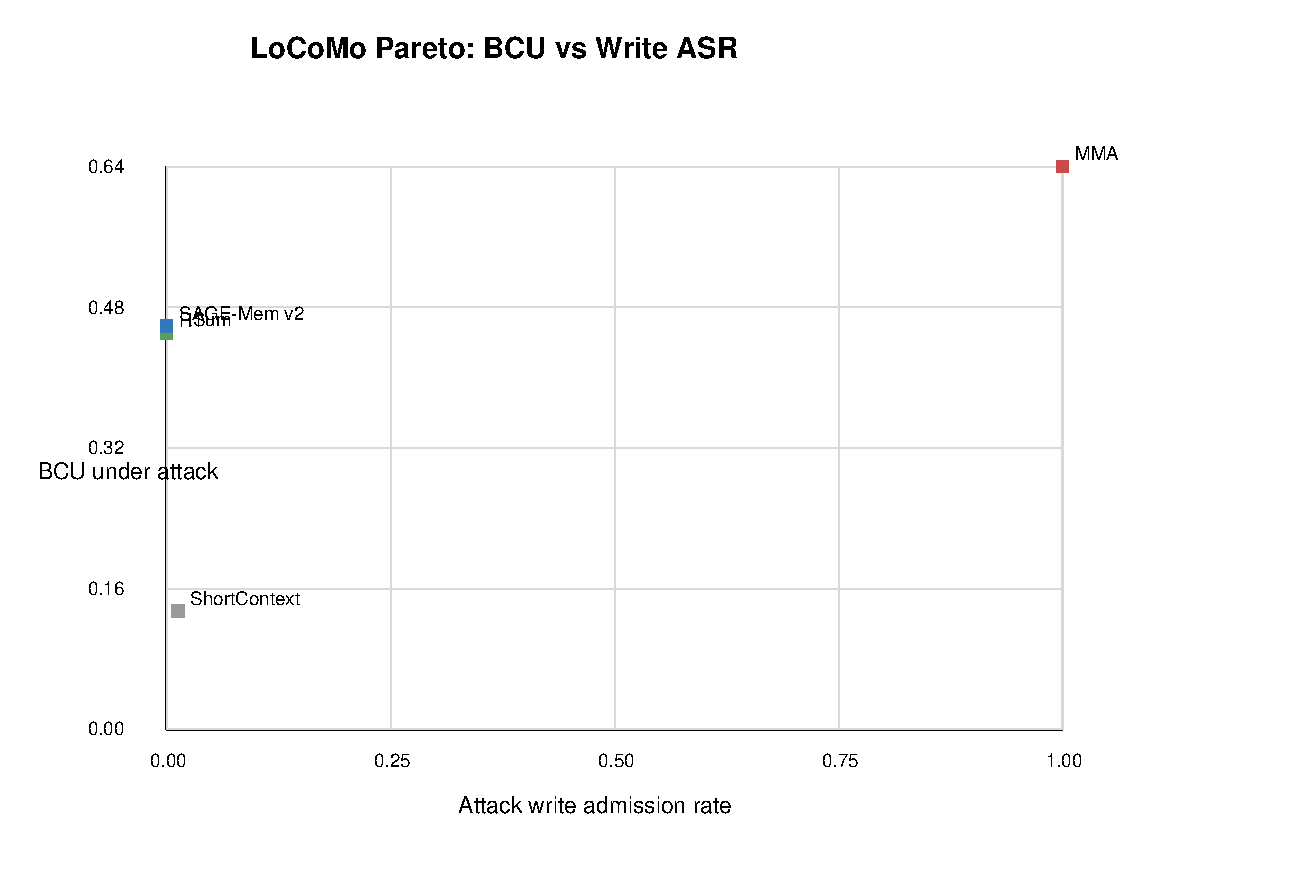
\includegraphics[width=\columnwidth]{pareto_locomo_bcu_vs_write_asr.pdf}
\caption{Integrity--utility Pareto frontier on the main LoCoMo benchmark. Retrieval-time MMA occupies the high-utility / high-admission region, while SAGE-Mem occupies the low-admission region with lower benign completion under attack.}
\label{fig:pareto-locomo}
\end{figure}

\begin{figure}[t]
\centering
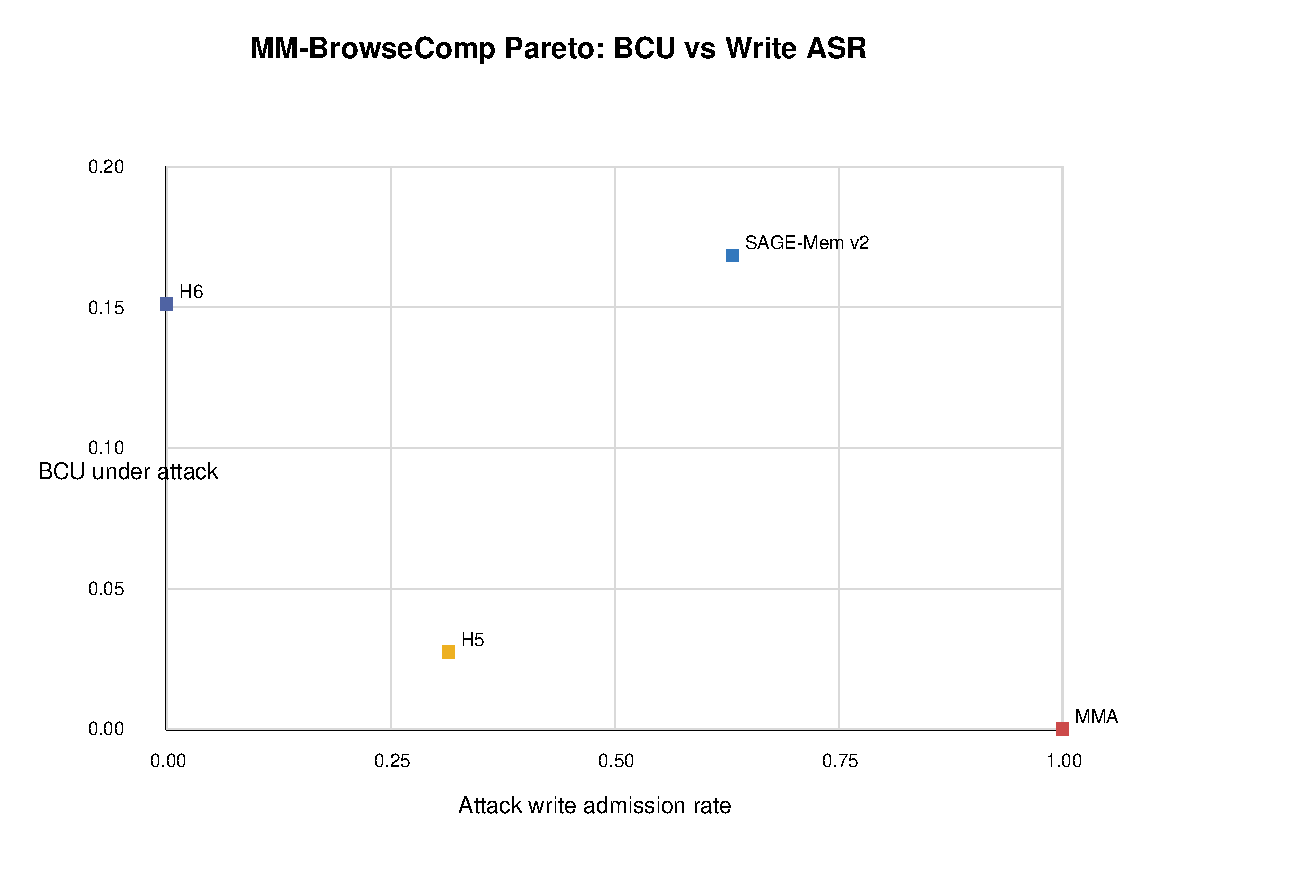
\includegraphics[width=\columnwidth]{pareto_browsing_bcu_vs_write_asr.pdf}
\caption{Integrity--utility Pareto frontier on grouped MM-BrowseComp. SAGE-Mem-BrowseGuard reaches the zero-admission, zero-retrieval-contamination corner while maintaining near-clean utility; SAGE-Mem-Browse remains vulnerable on the adaptive browser overwrite track.}
\label{fig:pareto-browsing}
\end{figure}



\subsection{Novelty Relative to Prior Work}

The novelty is not simply another write-time filter. The contribution is the combination of:

\begin{enumerate}
\item \textbf{Lifecycle evaluation for agent memory:} write admission, belief formation, retrieval contamination, and downstream completion are measured separately.
\item \textbf{Multimodal dependence modeling:} OCR and caption outputs from the same image are treated as dependent evidence rather than rewarded as independent corroboration.
\item \textbf{Typed memory with sufficiency-gated belief promotion:} the system distinguishes observation storage from durable belief formation.
\item \textbf{Honest benchmarking methodology:} we explicitly introduce an adaptive attack variant (\texttt{fact\_overwrite\_adaptive}) to test whether browsing defenses generalize beyond one overwrite rendering, and disclose that a provenance-only browser prior is insufficient on this benchmark.
\item \textbf{SAGE-Mem-BrowseGuard:} a browser-specific write-time gate combining an answer-memory write restriction with composite semantic suspicion scoring over page-group anomaly, corroboration deficit, and channel history. The answer-memory restriction is the dominant mechanism; secondary signals provide defense-in-depth.
\end{enumerate}

These novelty claims should be read with appropriate scope. The LoCoMo setting is controlled rather than fully naturalistic, the utility gap versus MMA is real, and BrowseGuard's strongest mechanism is the structured browser claim gate rather than the secondary anomaly signals alone. Framed this way, the paper makes a clear and defensible workshop contribution.



\section{Implications for ML Systems in the Global South}

The empirical story in this paper is especially relevant for deployments that operate in unreliable and low-trust information ecosystems. In many Global South contexts, ML systems must work with scanned records, photographed forms, multilingual or code-switched text, informal web content, and tool outputs with limited provenance. Human verification may be expensive, bandwidth may be intermittent, and upstream data quality may vary substantially across institutions. Under these conditions, persistent memory is useful because it preserves context across long interactions, but it is also risky because low-quality or adversarial information can become durable state.

Three implications follow. First, memory integrity may matter more than maximizing one-step accuracy. In public-service settings such as benefits administration, logistics coordination, health support, or digital public infrastructure, a system that answers slightly more questions correctly on average may still be undesirable if it stores and later reuses unsupported information. Second, noisy multimodal inputs should be treated as a structural condition rather than an edge case. The VPI and noisy-modality experiments capture common failure modes of low-resource deployments: OCR errors from old scans, image-derived text from low-quality cameras, and repeated evidence produced by one underlying source. Third, low-trust web evidence requires stricter write-time controls than generic tool outputs. The browsing results show that externally sourced factual claims should not be written into durable answer-bearing memory under the same trust assumptions as internal tool outputs.

More broadly, the paper argues that \emph{memory governance is part of making advanced ML systems usable in under-resourced environments}. Cleaner writes can reduce repeated manual correction, lower the downstream burden on retrieval reranking, and make long-horizon systems more dependable when trusted data infrastructure is limited.

\section{Limitations}

\begin{itemize}
\item \textbf{Trusted orchestration assumption.} Source labels are assumed correct.
\item \textbf{Utility tradeoff.} Retrieval-time baselines preserve more immediate QA utility. This is the expected cost of conservative write-time governance rather than an artifact to hide; the appropriate operating point depends on whether deployment prioritizes short-term answer rate or persistent memory integrity.
\item \textbf{Controlled rather than field-deployed evaluation.} LoCoMo is controlled, and MM-BrowseComp is only a proxy for low-trust web and document ecosystems. We do not claim evaluation on real-world Global South datasets or field deployments.
\item \textbf{Compute and infrastructure assumptions.} Our current setup does not model low-compute, intermittent-connectivity, or on-device constraints that matter in many low-resource deployments.
\item \textbf{Limited multilingual validation.} Although the motivation includes heterogeneous and low-quality inputs, we have not yet evaluated SAGE-Mem at scale on multilingual document collections, code-switched text, or region-specific web ecosystems.
\item \textbf{SAGE-Mem-Browse is a weak baseline rather than a robust browsing defense.} In the browsing rerun, the provenance-only browser prior does not materially improve over generic SAGE-Mem on write admission and remains highly vulnerable on the overwrite benchmark.
\item \textbf{SAGE-Mem-BrowseGuard scope.} The structured browser claim gate blocks browser-sourced factual assertion writes by content-type classification. Attacks that target other memory types or arrive on non-browser channels rely on secondary scoring and trust thresholds. Broader web attacks such as hidden instructions, multi-page contradictions, and login-gated evidence remain outside current evidence.
\item \textbf{Module separability is setting-dependent.} Bayes calibration is most clearly supported by the noisy/missing-modality run, not the main suite.
\end{itemize}

\section{Future Work}

Future work should strengthen the method along two axes: richer multimodal semantics and closer alignment with deployment constraints in under-resourced environments.

The most important scientific direction is to move from write-time multimodal governance toward \textbf{write-time multimodal verification}. Our results show that memory systems should not mistake dependent channels for independent corroboration, and that browser-sourced factual claims require stricter write-time treatment than generic tool output. What remains to be shown is a cross-modal verifier that adjudicates disagreements among OCR, caption, page text, and trusted memory state.

The most important deployment direction is to validate these ideas on real data pipelines that reflect Global South conditions: multilingual document collections, OCR-heavy administrative workflows, mobile-image ingestion, and public web ecosystems with inconsistent provenance. Low-compute adaptations are also important. The method is motivated by settings where verification resources are limited, but we have not yet optimized for edge or intermittently connected environments.

The most important benchmark direction is to broaden the browsing attack surface beyond direct browser-sourced answer overwrites. A richer benchmark should include hidden-instruction attacks, multi-page contradictions, control-memory attacks, and cases where the answer lives primarily in visual or dynamic web content. Finally, future work should investigate calibration strategies that preserve more benign evidence without sacrificing memory integrity, since overly conservative systems may reject scarce but valuable context in low-resource settings.




\bibliography{references}
\bibliographystyle{icml2026}

\end{document}
